\section{Experimental Setup}
\label{sec:experiments}

This section describes the simulated environment, the baselines, the
training setup and the evaluation protocol, and reports the empirical
results with proper statistical summaries.


\subsection{Dataset and simulation environment}
\label{subsec:dataset}

Direct online access to Philips France's contractual inventory is subject
to confidentiality and operational constraints, so we do not conduct
training on the production systems. Instead, we build a \emph{simulation
environment} whose parameter distributions are chosen to reproduce the
qualitative characteristics of a hospital-equipment installed base:
coverage levels, contract durations, contractual costs, and equipment
risk levels. This environment plays the role of both dataset and
interaction simulator, which guarantees full experimental reproducibility
and avoids any exposure of sensitive data.

Each episode represents a single piece of medical equipment tracked over
a finite horizon of $T = 120$ daily time steps. At reset, the
environment randomly draws: a remaining time before current coverage
expiration within $[5, 30]$ days, a contract-cost level with three
modalities (low, medium, high), and a risk level with three modalities
(low, medium, high). The equipment is initially covered.

The state space is a four-dimensional vector combining the coverage
status, the number of days before expiration of the current coverage,
the contract-cost level and the risk level of the equipment. All
components are normalized to the unit interval before being fed to the
policy.

The action space is discrete and contains three decisions: do nothing,
renew the contract, or extend the warranty. Renewal resets coverage to a
fixed duration ($30$ days), whereas warranty extension adds an extra
duration ($30$ days, capped at $60$) at a reduced cost, conditional on
an active contract being in place.

The dynamics decrement the remaining time before expiration by one day
at each step. Expiration triggers a transition to the uncovered state
and a one-shot penalty. Failures are sampled at each step with a
probability increasing with the risk level; failures occurring on
uncovered equipment are penalized more heavily than others. The reward
function aggregates six components: a continuous coverage bonus, a bonus
for renewals performed close to expiration, a renewal or extension cost
indexed on the contract-cost level, a penalty for overly early renewals,
a continuous non-coverage penalty, and a one-shot expiration penalty.
Coefficients are chosen so that the per-step reward remains in a
numerically stable range while preserving a clear ordering between
desirable and undesirable actions.


\subsection{Baseline policies}
\label{subsec:baselines}

We compare the PPO agent with three complementary baselines.
The first is a uniformly random policy over the three actions,
which sets a lower performance bound. The second is a rule-based heuristic
reflecting operational practice (Section~\ref{subsec:sensitivity})
with a nominal threshold of five days.

The third is the greedy policy computed by synchronous value iteration on
the expected-reward tabular MDP of Section~\ref{subsec:vi-baseline}.
Throughout we refer to it as ``VI~(exp.)'': discounted Bellman-optimal
\emph{in expectation}, rolled out with the identical simulator as every other
baseline.\footnote{Welch's two-sided test on per-episode rewards between
VI and heuristic returns $t \approx 0.036$, $p \approx 0.97$ ($n{=}100$ shared seeds),
which is consistent with the hypothesis that threshold rules saturate the Bellman-optimal frontier in expectation here.}


\subsection{Architecture and training setup}
\label{subsec:training}

The policy and value function share a two-layer fully connected encoder
of width $64$ with $\tanh$ activations, followed by two linear heads: a
softmax head over the three actions and a scalar value head.
Observations are normalized online through a running estimate of the
mean and variance (using Welford's algorithm), then clipped to the
interval $[-5, 5]$ before being fed to the network.

Training uses PPO with Generalized Advantage Estimation (GAE). At each
iteration, a full episode is collected under the current policy, the
advantage is computed, and the policy-value pair is updated for four
passes over mini-batches of size $64$. Advantages are normalized per
batch. The objective combines PPO's clipped loss, a squared value loss
and an entropy bonus encouraging exploration.

Hyperparameters are summarized in Table~\ref{tab:hparams}. They follow
standard PPO values, with a slightly higher entropy coefficient to
maintain exploration over the considered training horizon.

\begin{table}[h]
\centering
\begin{tabular}{lc}
\toprule
Hyperparameter & Value \\
\midrule
Number of episodes            & $3{,}000$ \\
Episode horizon               & $120$ days \\
Learning rate                 & $3 \times 10^{-4}$ \\
Discount factor               & $0.99$ \\
GAE parameter                 & $0.95$ \\
Clip range                    & $0.2$ \\
Optimization epochs           & $4$ \\
Mini-batch size               & $64$ \\
Hidden dimension              & $64$ \\
Entropy coefficient           & $0.02$ \\
Value coefficient             & $0.5$ \\
Observation clipping          & $[-5, 5]$ \\
\bottomrule
\end{tabular}
\caption{Training hyperparameters.}
\label{tab:hparams}
\end{table}


\subsection{Evaluation protocol}
\label{subsec:eval-protocol}

Every $100$ training episodes, the current policy is evaluated in
deterministic mode (argmax action selection) over $20$ episodes sharing
fixed simulation seeds. The best policy in terms of evaluation reward is
retained and restored at the end of training.

The \emph{final} comparison with the baseline policies is conducted on
a separate and larger pool of $100$ simulation seeds, shared across every
policy, so that they face identical contract and failure trajectories.
This procedure neutralizes the stochastic variance of the environment and
enables a statistically sound comparison between random, heuristic, VI and
learned controllers. We report,
for every metric and every policy, the sample mean, the sample standard
deviation and a two-sided $95\%$ confidence interval on the mean
computed with Student's $t$-distribution ($\mathrm{df}=99$). Welch's tests
against PPO include both the heuristic and the VI baseline reported in Table~\ref{tab:results}.

Three metrics summarize the performance of a policy on the evaluation
set: the \emph{mean cumulative reward} per episode, which aggregates all
reward components and is to be maximized; the \emph{mean number of
uncovered steps}, which measures the time the equipment remains without
active coverage and is to be minimized; and the \emph{mean number of
uncovered failures}, which quantifies costly events that occur outside
any contract, whose minimization is an operational priority.


\subsection{Results}
\label{subsec:results}

The performance on $100$ shared evaluation seeds
is reported in Table~\ref{tab:results}. We report the sample mean, the
sample standard deviation, and a two-sided $95\%$ confidence interval on
the mean.

\begin{table}[h]
\centering
\footnotesize
\setlength{\tabcolsep}{3.5pt}
\begin{tabular}{lcccc}
\toprule
Metric & Random & Heuristic & PPO & VI (exp.) \\
\midrule
Cumulative reward    &
    $-241.44 \pm 92.66$                        &
    $\phantom{-}58.06 \pm \phantom{0}3.93$     &
    $\phantom{-}44.83 \pm 20.05$               &
    $\phantom{-}58.08 \pm \phantom{0}3.96$       \\
                                                &
    $[-259.60,\,-223.28]$                      &
    $[\phantom{-0}57.29,\,\phantom{-0}58.84]$  &
    $[\phantom{-0}40.90,\,\phantom{-0}48.76]$  &
    $[\phantom{-0}57.31,\,\phantom{-0}58.86]$    \\
\addlinespace
Uncovered steps      &
    $\phantom{-00}0.00 \pm \phantom{0}0.00$    &
    $\phantom{-00}0.00 \pm \phantom{0}0.00$    &
    $\phantom{-00}1.12 \pm \phantom{0}1.81$    &
    $\phantom{-00}0.00 \pm \phantom{0}0.00$      \\
                                                &
    $[\phantom{-0}0.00,\,\phantom{-00}0.00]$   &
    $[\phantom{-0}0.00,\,\phantom{-00}0.00]$   &
    $[\phantom{-0}0.77,\,\phantom{-00}1.47]$   &
    $[\phantom{-0}0.00,\,\phantom{-00}0.00]$     \\
\addlinespace
Uncovered failures   &
    $\phantom{-00}0.00 \pm \phantom{0}0.00$    &
    $\phantom{-00}0.00 \pm \phantom{0}0.00$    &
    $\phantom{-00}0.11 \pm \phantom{0}0.40$    &
    $\phantom{-00}0.00 \pm \phantom{0}0.00$      \\
                                                &
    $[\phantom{-0}0.00,\,\phantom{-00}0.00]$   &
    $[\phantom{-0}0.00,\,\phantom{-00}0.00]$   &
    $[\phantom{-0}0.03,\,\phantom{-00}0.19]$   &
    $[\phantom{-0}0.00,\,\phantom{-00}0.00]$     \\
\bottomrule
\end{tabular}
\caption{Performance comparison over $100$ evaluation episodes with
         shared seeds ($\text{seeds} = 2000, \ldots, 2099$). Each cell
         reports $\text{mean} \pm \text{SD}$ on the first line and the
         $95\%$ confidence interval on the mean (Student's $t$,
         $\mathrm{df}=99$) on the second. Values are regenerated by
         \texttt{main.py}; column \emph{VI (exp.)} is the greedy policy from
         value iteration (\texttt{dp\_solver.py}) on the expected MDP.}
\label{tab:results}
\end{table}

\paragraph{Main finding.}
The heuristic attains a mean reward of $58.06$ and PPO attains $44.83$;
the gap is far outside the respective $95\%$ confidence intervals.
Welch's test on per-episode rewards yields $t = -6.48$, $p < 0.0001$
($\mathrm{df} \approx 107$). The tabular Bellman policy (VI) attains
$58.08 \pm 3.96$, statistically indistinguishable from the heuristic
(Welch $t \approx 0.04$, $p \approx 0.97$), so the latter should be
understood as \emph{co-optimal} with the exact finite-horizon tabulation
of Section~\ref{subsec:vi-baseline}, not as an arbitrary engineering
baseline. PPO's gap is therefore a gap to the Bellman--optimal frontier of
this toy MDP, driven by function approximation and finite training rather
than by a weak reference policy.

PPO's episode-level standard deviation ($20.05$) is roughly five times
that of either co-optimal baseline ($\approx 4$), underscoring reliability
concerns on identical seeds. The random policy at $-241.44$ remains a
coarse lower bound.

Finally, parallel Welch tests \emph{PPO vs VI} (reported with full
precision in \texttt{results.md} after each run) confirm the same
significance pattern as \emph{PPO vs heuristic}: the learned policy is
far from the tabular optimum on average.

\paragraph{A counter-intuitive but well-explained random baseline.}
The random policy obtains a strongly negative reward despite recording
zero uncovered steps and zero uncovered failures in every evaluated
episode. This apparently counter-intuitive result stems from the
structure of the action space: by drawing uniformly among the three
decisions, two of which---renew and extend---preserve or restore
coverage, the random agent mechanically keeps contracts active but
accumulates prohibitive contractual costs. The absence of a strategy
thus manifests as expensive over-coverage rather than under-coverage,
and confirms that the sole metric of uncovered steps does not fully
capture the quality of a policy.

\paragraph{PPO learns a competent but unstable policy.}
PPO reaches a clearly positive mean reward and demonstrates that a
standard policy-gradient procedure is able to learn, from interactions
with the simulator alone, a policy that keeps the equipment covered
during the overwhelming majority of each episode ($1.12$ uncovered step
and $0.11$ uncovered failure per episode on average) while limiting
renewal costs. The policy is not competitive with the heuristic in mean
reward, however, and its high variance indicates that convergence is
not fully stable within the $3{,}000$-episode training budget: a small
fraction of evaluation episodes yields rewards well below the bulk of
the distribution, dragging the mean down. The residual gap to the
heuristic is analyzed in detail in Section~\ref{sec:discussion}; in
short, it reflects the fact that the optimal policy of the considered
environment is exactly representable as a one-dimensional threshold
rule, which the heuristic encodes by construction and which PPO has to
rediscover through noisy exploration.


\subsection{Sensitivity analysis: heuristic threshold}
\label{subsec:sensitivity}

A natural concern is that the strong performance of the heuristic might
come from a specific, favourable choice of its renewal threshold.
Table~\ref{tab:sensitivity} reports the mean reward of the heuristic for
five values of the threshold, evaluated on the same $100$ shared seeds.

\begin{table}[h]
\centering
\small
\begin{tabular}{lccccc}
\toprule
Threshold (days) & $3$ & $5$ & $7$ & $10$ & $15$ \\
\midrule
Mean reward $\pm$ SD &
    $58.06 \pm 3.93$ &
    $58.06 \pm 3.93$ &
    $49.98 \pm 4.00$ &
    $49.74 \pm 4.23$ &
    $49.14 \pm 4.62$ \\
$95\%$ CI &
    $[57.29,\,58.84]$ &
    $[57.29,\,58.84]$ &
    $[49.20,\,50.76]$ &
    $[48.91,\,50.57]$ &
    $[48.24,\,50.04]$ \\
\bottomrule
\end{tabular}
\caption{Heuristic renewal-threshold sensitivity on the same $100$
         shared seeds as Table~\ref{tab:results}. Thresholds of $3$
         and $5$ induce an identical policy in practice because
         contracts rarely reach the $[0, 3]$ days-to-expiration range
         without being renewed first.}
\label{tab:sensitivity}
\end{table}

Three observations emerge from the sweep. First, the heuristic's peak
is flat: thresholds of $3$ and $5$ produce exactly the same mean
reward ($58.06$) because episodes rarely observe $\mathrm{days\_to\_exp}
\in [0, 3]$ in practice. Second, the heuristic is \emph{robust} across
its operating range: the largest observed loss is only $8.9$ reward
units between the peak and threshold $15$, corresponding to a $15\%$
relative degradation. Third, the learned PPO policy at $44.83 \pm 20.05$ lies well below
VI ($58.08 \pm 3.96$) and even the weakest heuristic instantiation
($49.14$, threshold $15$); only the pessimistic extreme of PPO's
confidence interval marginally overlaps the weakest heuristic regime.
A longer training budget, a richer observation space, or the
regularisation strategies discussed in Section~\ref{sec:discussion}
remain candidate leverage points because the deficits are sizeable
relative to both the analytic optimum and plausible rule perturbations.

The residual message is methodological: thresholds are swept to bound
\textbf{engineering} ambiguity, whereas VI resolves \textbf{Bellman}
optimality in expectation and shows that ambiguity is negligible between
those two viewpoints here.


\subsection{Ablations, longer training and alternative RL methods}
\label{subsec:further-exp}

\textbf{Ablations.} Systematic grids over PPO internals (entropy
coefficients, clipping range, optimisation epochs, learning-rate
schedules) and reward-shape coefficients tighten confidence that an
implementation is faithful rather than brittle. Recording learning
curves for each configuration would quantify stability of the plateau
highlighted in Section~\ref{subsec:training_dynamics}.

\textbf{Longer horizons.} Extending optimisation to $10^4$--$10^5$
episodes is a pragmatic stress test for diminishing returns on this
architecture: value iteration delineates attainable performance exactly,
so divergence from VI after arbitrarily long optimisation would quantify
persisting approximation error beyond finite budgets.

\textbf{Alternative algorithms.} Off-policy methods (soft actor--critic,
quantile-based critics) or replay-based value learners (DQN variants) may
lower variance in principle, yet they do not remove the fundamental
issue that the tabular Bellman solution is already near-trivially
encoded by co-optimal threshold rules in the present toy MDP. We defer
comprehensive head-to-head comparisons to future work on enriched state
spaces where such rules lose their near-optimality.


\subsection{Training dynamics}
\label{subsec:training_dynamics}

\begin{figure}[h]
    \centering
    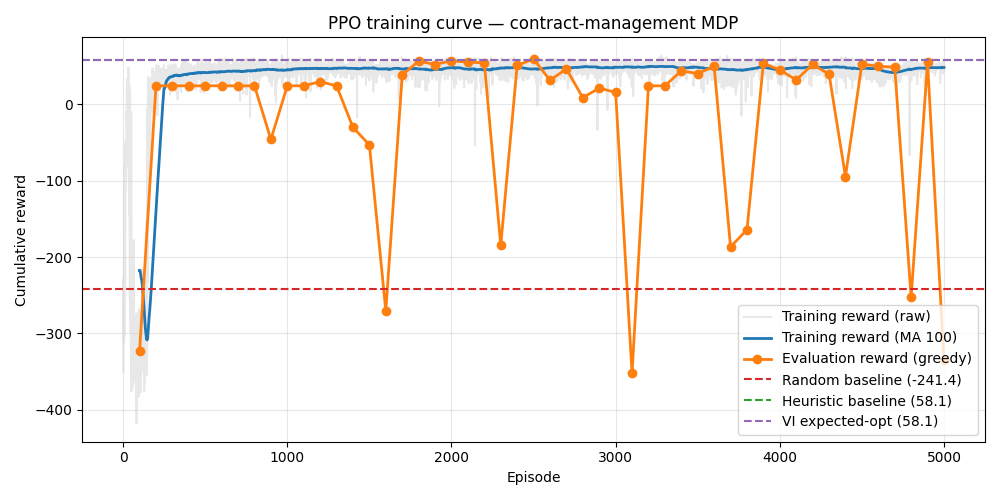
\includegraphics[width=0.8\linewidth]{figures/training_curve.png}
    \caption{Training dynamics of the PPO agent. The light gray trace
             shows the raw per-episode training reward, the solid blue
             line its moving average, and the orange markers the greedy
             evaluation reward measured every $100$ episodes on the
             fixed training-time evaluation pool. Dashed horizontal
             lines mark the random baseline, heuristic mean and tabular VI
             mean from Table~\ref{tab:results}.}
    \label{fig:training_curve}
\end{figure}

Figure~\ref{fig:training_curve} summarizes the training dynamics. Four
observations deserve to be highlighted. First, during the initial
$200$ episodes the training reward is strongly negative and close to
the random-policy level, reflecting the cost of exploration before the
policy discovers the coverage semantics. Second, a clear upward
inflection is visible between episodes $200$ and $500$, during which
the agent simultaneously reduces uncovered periods and limits
expensive over-coverage; the moving average of the training reward
crosses the random baseline and then the zero line in this interval.
Third, after roughly $600$ episodes the moving average plateaus in the
range $[40, 48]$, well below both co-optimal baselines at $\approx 58.1$
(see heuristic and VI means in Table~\ref{tab:results}): training settles
far from the Bellman reference, and longer horizons alone constitute an
engineering rather than principled remedy once VI is known. Fourth, and crucially for the
interpretation of the results, the per-episode greedy evaluation
(orange markers) is highly \emph{volatile}: it oscillates between
$+55$ and $-194$ well into the second half of training, which directly
explains the large episode-to-episode variance ($\text{SD} = 20.05$)
reported in Table~\ref{tab:results}. These observations jointly
support the interpretation developed in
Section~\ref{sec:discussion}.


\subsection{Scope of the empirical claims}
\label{subsec:scope}

The results in this section are obtained in a deliberately simplified
simulation environment whose distributions are controlled by a handful
of parameters. They therefore do not directly entail the performance
achievable in production, where additional factors---portfolio
heterogeneity, global budget constraints, partial observability,
non-stationary dynamics---that are absent from the present framework
come into play. Within this scope, the results motivate a sharper claim than ``PPO loses
against a heuristic'': VI shows the heuristic coincides---up to Monte Carlo
noise---with an exact Bellman policy on an augmented finite MDP, whereas PPO remains
almost $13$ reward units behind on average $(p \ll 10^{-4})$ with five times larger
reward variance across identical seeds.

We interpret this as evidence that reinforcement learning is misaligned when
evaluation metrics favour parsimonious expert rules coinciding with analytic optima,
not evidence that RL is incapable of exploiting richer structure absent from our toy model.
